\documentclass{sigchi-ext}
% Please be sure that you have the dependencies (i.e., additional
% LaTeX packages) to compile this example.
\usepackage[T1]{fontenc}
\usepackage{textcomp}
\usepackage[scaled=.92]{helvet} % for proper fonts
\usepackage{graphicx} % for EPS use the graphics package instead
\usepackage{balance}  % for useful for balancing the last columns
\usepackage{booktabs} % for pretty table rules
\usepackage{ccicons}  % for Creative Commons citation icons
\usepackage{ragged2e} % for tighter hyphenation

% Some optional stuff you might like/need.
% \usepackage{marginnote}
% \usepackage[shortlabels]{enumitem}
% \usepackage{paralist}
% \usepackage[utf8]{inputenc} % for a UTF8 editor only

%% EXAMPLE BEGIN -- HOW TO OVERRIDE THE DEFAULT COPYRIGHT STRIP --
\copyrightinfo{This article is licensed under the Creative Commons \\
Attribution 4.0 International license (CC BY 4.0). You are free to share\\
and adapt this work, provided you attribute the authors and leave this \\ copyright notice intact.
 {\emph{CSCW'18}}, November 3-7, 2018, Jersey City, NJ, USA. \\
 https://doi.org/XXXXX/XXXXX}

% Paper metadata (use plain text, for PDF inclusion and later
% re-using, if desired).  Use \emtpyauthor when submitting for review
% so you remain anonymous.
\def\plaintitle{Community Literacy of Machine Learning: Engineering practical support for participatory design and auditing}
\def\plainkeywords{Algorithm; Fairness; Transparency; Wikipedia; Collaboration; Participatory design; Auditing}
\def\plaingeneralterms{Algorithm, Fairness, Transparency, Wikipedia, Collaboration, Participatory, Auditing}
\title{Community Literacy of Machine Learning: Engineering practical support for participatory design and auditing}


\def\plainauthor{Aaron Halfaker and Stuart Geiger}
\def\emptyauthor{}

\numberofauthors{2}
% Notice how author names are alternately typesetted to appear ordered
% in 2-column format; i.e., the first 4 autors on the first column and
% the other 4 auhors on the second column. Actually, it's up to you to
% strictly adhere to this author notation.
\author{%
  \alignauthor{%
    \textbf{Aaron Halfaker}\\
    \affaddr{Wikimedia Research} \\
    \affaddr{San Francisco, CA, USA} \\
    \email{ahalfaker@wikimedia.org} }\alignauthor{%
    \textbf{Stuart Geiger}\\
    \affaddr{Univ. of California, Berkely}\\
    \affaddr{Berkeley Inst. of Data Science}\\
    \affaddr{Berkeley, CA, USA}\\
    \email{sgeiger@gmail.com} } }


% Make sure hyperref comes last of your loaded packages, to give it a
% fighting chance of not being over-written, since its job is to
% redefine many LaTeX commands.
\definecolor{linkColor}{RGB}{6,125,233}
\hypersetup{%
  pdftitle={\plaintitle},
%  pdfauthor={\plainauthor},
  pdfauthor={\emptyauthor},
  pdfkeywords={\plainkeywords},
  bookmarksnumbered,
  pdfstartview={FitH},
  colorlinks,
  citecolor=black,
  filecolor=black,
  linkcolor=black,
  urlcolor=linkColor,
  breaklinks=true,
}

% \reversemarginpar%

\begin{document}

%% For the camera ready, use the commands provided by the ACM in the Permission Release Form.
%\CopyrightYear{2007}
%\setcopyright{rightsretained}
%\conferenceinfo{WOODSTOCK}{'97 El Paso, Texas USA}
%\isbn{0-12345-67-8/90/01}
%\doi{http://dx.doi.org/10.1145/2858036.2858119}
%% Then override the default copyright message with the \acmcopyright command.
%\copyrightinfo{\acmcopyright}

\maketitle

% Uncomment to disable hyphenation (not recommended)
% https://twitter.com/anjirokhan/status/546046683331973120
\RaggedRight{}

% Do not change the page size or page settings.
\begin{abstract}
Algorithmic systems---from rule-based bots to machine learning classifiers---have a long history of supporting the essential work of content moderation and other curation work in peer production projects.  From counter-vandalism to task routing, basic machine prediction has allowed open knowledge projects like Wikipedia to scale to the largest encyclopedia in the world, while maintaining quality and consistency.  However, conversations about what quality control should be and what role algorithms should play have generally been led by the expert engineers who have the skills and resources to develop and modify these complex algorithmic systems. In this paper, we describe ORES: an algorithmic scoring service that supports real-time scoring of wiki edits using multiple independent classifiers trained on different datasets. ORES decouples three activities that have typically all been performed by engineers: choosing or curating training data, building models to serve predictions, and developing interfaces or automated agents that act on those predictions. This meta-algorithmic system was designed to open up socio-technical conversations about algorithmic systems in Wikipedia to a broader set of participants.
\end{abstract}

\keywords{\plainkeywords}

\section{Introduction}
Wikipedia---the free encyclopedia that anyone can edit---faces many challenges in maintaining the quality of its articles and sustaining the volunteer community of editors. The people behind Wikipedia have long relied on automation, bots, expert systems, recommender systems, human-in-the-loop assisted tools, and machine learning to help moderate and manage content. The issues around artificial intelligence in Wikipedia are as complex as those facing other large-scale user-generated content platforms, as well as traditional organizations that must make and manage decisions at scale. And like in those organizations, Wikipedia's automated classifiers are raising new and old issues about truth, power, responsibility, openness, and representation.

Yet Wikipedia's approach to AI has long been different than in corporate or governmental contexts typically discussed in emerging fields like Fairness, Accountability, and Transparency in Machine Learning (FATML) or Critical Algorithms Studies (CAS). The volunteer community of editors has strong ideological principles of openness, decentralization, and consensus-based decision-making. The paid staff at the non-profit Wikimedia Foundation are not tasked with making editorial decisions about content\footnote{Except in rare cases, such as content that violates U.S. law}. This is instead the responsibility of the volunteer community, where a self-selected set of developers build tools, bots, and advanced technologies in broad consultation with the community. Even though Wikipedia's longstanding socio-technical system of algorithmic governance is far more open, transparent, and accountable than most platforms operating at Wikipedia's scale, ORES\footnote{\url{https://ores.wikimedia.org} and \url{http://enwp.org/:mw:ORES}}, the system we present in this paper, pushes even further on the crucial issue of who is able to participate in the development and use of advanced technologies.

\section{The politics of algorithms}
Algorithmic systems play increasingly crucial roles in the governance of social processes\cite{gillespie2014relevance}. Software algorithms are increasingly used in answering questions that have no single right answer and where prior human decisions used as training data can be problematic \cite{barocas2013governing}. Algorithms designed to support work change people's work practices, shifting how, where, and by whom work is accomplished\cite{crawford2016algorithm, zuboff1988age}. There are repeated calls to address power dynamics and bias through transparency and accountability \cite{diakopoulos2017algorithmic,sandvig2014auditing}. We cannot fully address the scale of concerns in this rapidly shifting literature, but we find inspiration in Kroll et al's discussion of the potential and limitations of auditing and transparency \cite{kroll2016accountable} and Geiger's call to go ``beyond opening up the black box\cite{geiger2017beyond}''.

We discuss a specific socio-political context---Wikipedia's algorithmic quality control and socialization practices---and the development of novel algorithmic systems for support of these processes.  ORES is a meta-algorithmic intervention aligned with Wikipedians' principles and practices: deploying a set of prediction algorithms as a service and leaving decisions about appropriation to the volunteer community.  Instead of training the single best classifier and implementing it in our own designs, we embrace public auditing, re-interpretations, and appropriations of our models' predictions as an \emph{intended} and \emph{desired} outcome.  Extensive work on technical and social ways to achieve fairness and accountability generally do not discuss this kind of socio-infrastructural intervention on communities of practice.

\section{The ORES system}
\begin{figure*}[h]
  \centering
  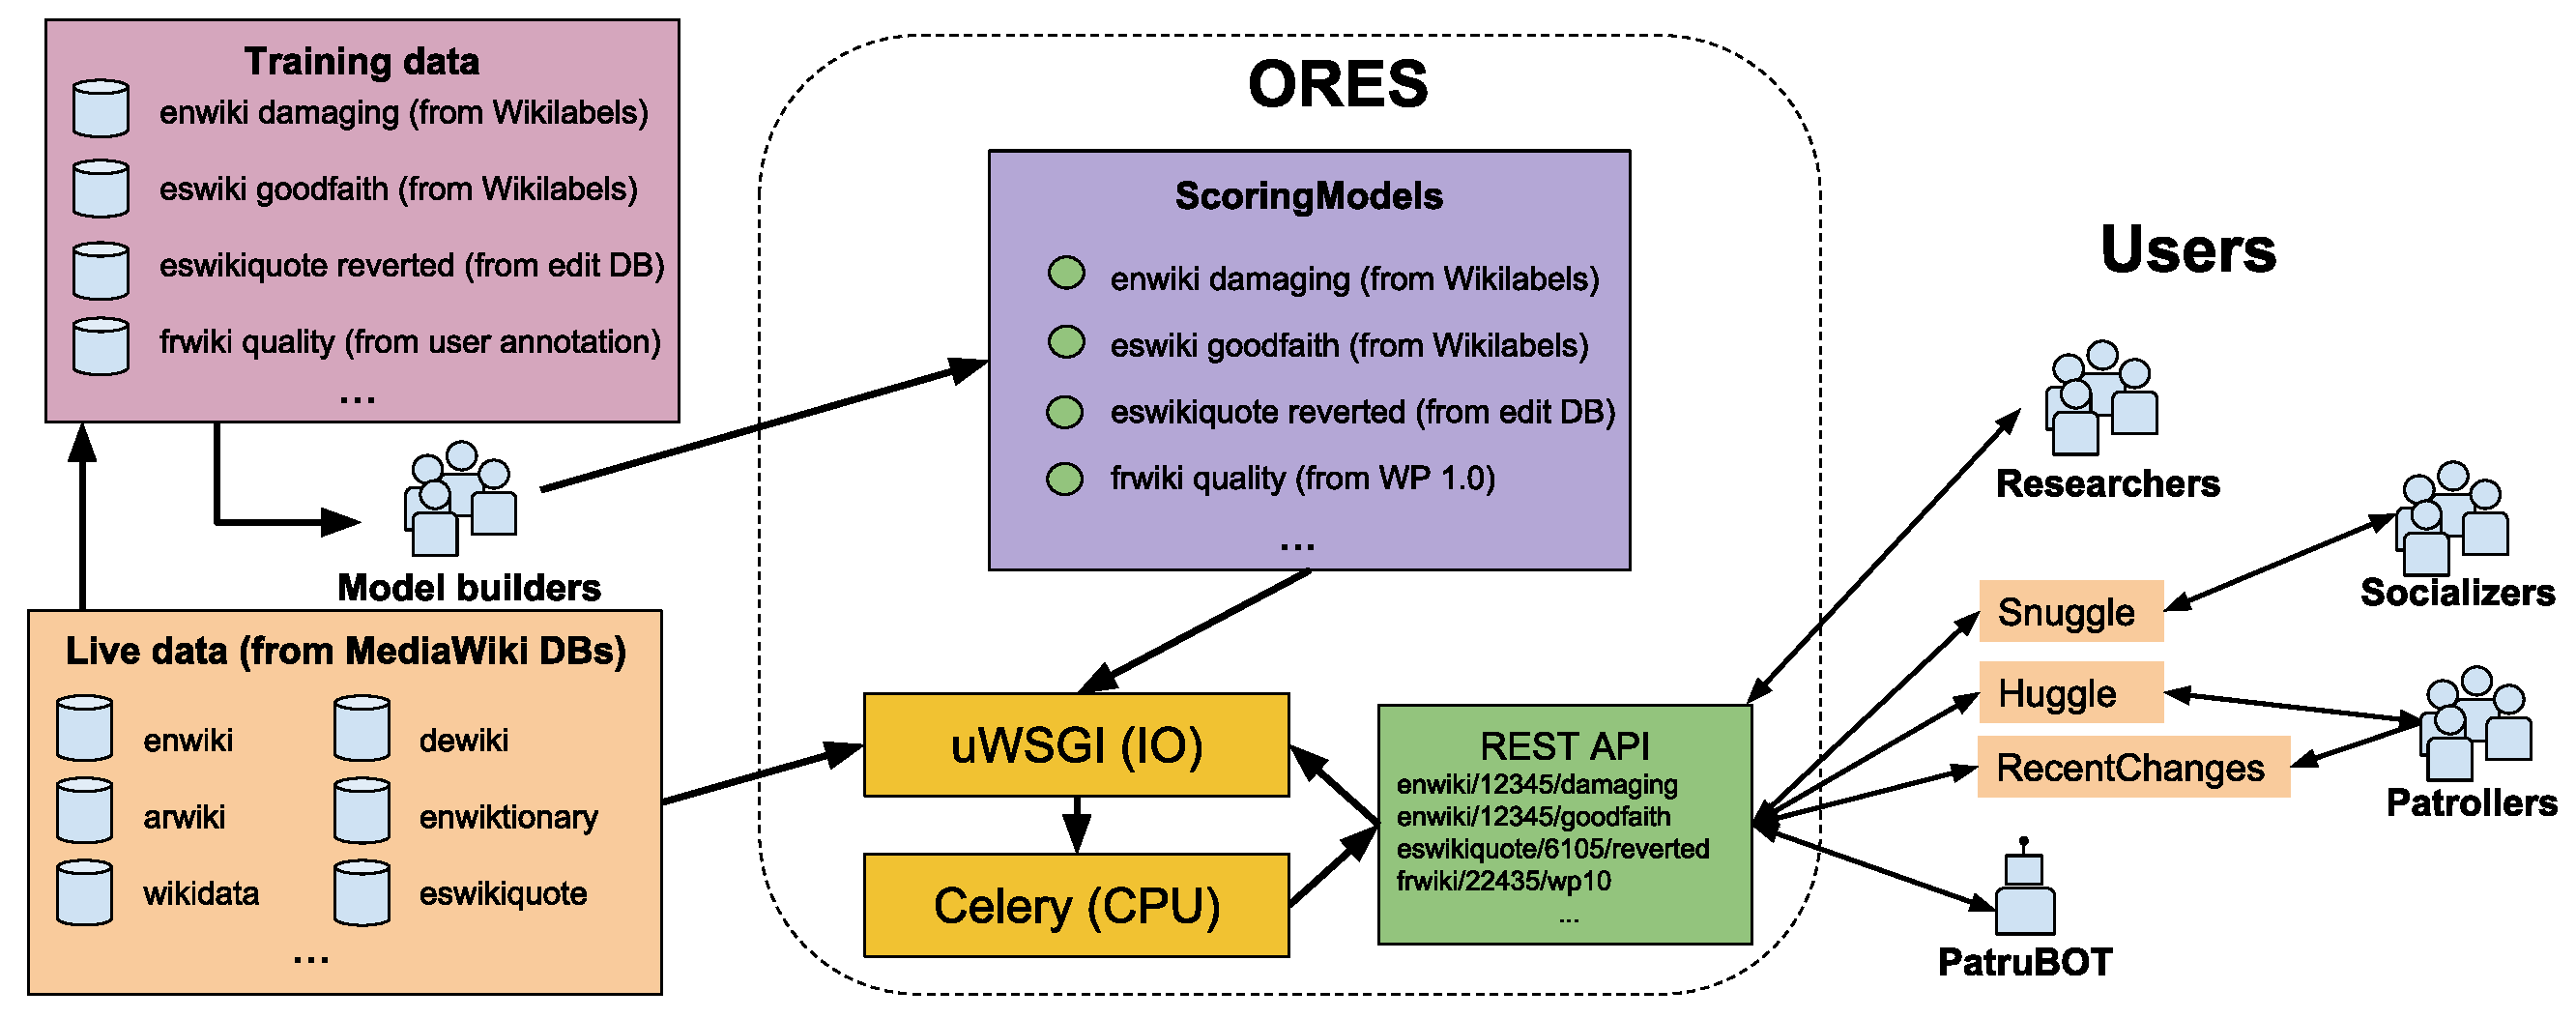
\includegraphics[width=.95\textwidth]{figures/ores_data_user_diagram}
  \caption{ORES conceptual overview.  Model builders design process for training ScoringModels from training data.  ORES hosts ScoringModels and makes them available to researchers and tool developers.}
  \label{fig:ores_data_user}
\end{figure*}

ORES is a collection of machine classifier models and an API.  These models are designed and engineered by a varied set of model builders (some external researchers and others by our own engineering team) using varied sources of \emph{training data}.  The models ORES hosts are engineered to support Wikipedian processes related to damage-detection, quality-assessment, and topic-routing, but the system is adaptable to a wide range of other models. To make these models available for users, ORES implements a containerized \emph{ScoringModel}, representing a fully trained and tested prediction model.  All \emph{ScoringModels} contain metadata about when the model was trained/tested and code for feature extraction. ORES provides access to ScoringModels via a RESTful HTTP interface and serves the predictions (JSON documents) to users.  We chose this service structure because Wikimedian tool developers (our target audience) are familiar with this RESTful API/JSON workflow, which is the standard endpoint for the MediaWiki API.

\section{Case Study: Patrolling/ORES (Italian Wikipedia)}
In this section, we describe a single case of collaborative auditing of ORES.  While there are many cases like this one, the case of Italian Wikipedia is an excellent example of collaborative grounded theory deployed \emph{in the field} to audit a machine prediction model. Italian Wikipedia was one of the first wikis where we deployed basic edit quality models.  Our local collaborator, who helped us develop the language specific features, User:Rotpunkt, created a page for ORES\footnote{\url{https://it.wikipedia.org/wiki/Progetto:Patrolling/ORES}} with a section for reporting false-positives (``falsi positivi'').

Within several hours, editors noticed some trends and collected false positives under different headers, representing themes they were seeing.  They were effectively performing an inductive, grounded theory-esque exploration of ORES errors, trying to identify themes and patterns. One theme was ``corrections to the verb for \emph{have}'' (``correzioni verbo avere'').  The word ``ha'' in Italian translates to the English verb ``to have''.  In English and many other langauges, ``ha'' is laughing, and adding ``ha'' repeatedly is a common type of vandalism seen in all languages of Wikipedia.  We'd built a common feature in the damage model called ``informal words'' that captured these types of patterns.  But in this case, it was clear that in Italian ``ha'' should not carry signal, while ``hahaha'' still should. Because of the work of Rotpunkt and his collaborators in Italian Wikipedia, we were able to recognize the source of this issue (a set of features intended to detect the use of \emph{informal language} in articles) and to remove ``ha'' from that list for Italian Wikipedia.

\section{Discussion}
Deploying ORES as a meta-algorithmic probe allows us to ask new questions about how people understand the algorithms that govern (or at least supplement the governance of) their spaces.  In the case above, while many participants in this analysis could not approach technical jargon of model fitness (e.g. \emph{precision} and \emph{recall}), they were able to effectively evaluate the behavior of their machine prediction model and to detect problematic trends (biases) that the model expressed.  The case of Italian Wikipedia and the way that people operate around ORES should prompt us to think about machine learning literacy and power differently.  This case shows that in one key respect (bias detection via crowd auditing), formal knowledge of machine learning was not necessary.  Instead, the openness of ORES (the ability to deterministically get the same prediction for the same edit and share that with others) made it possible for a large group of people to work together to build understanding.


\bibliographystyle{SIGCHI-Reference-Format}
\bibliography{refs}

\end{document}

%%% Local Variables:
%%% mode: latex
%%% TeX-master: t
%%% End:
